\toptitle{[ELEC-H-201] Électricité et électronique}{TP4}
\TPtitle{Électricité et électronique\vspace*{2mm}}{TP4:\vspace*{2mm}
Électronique numérique}

\frontpage{consignes4.tex}
\vspace{5cm}
\newpage

\section{Représentation des nombres en binaire}
\subsection{Système décimal (base 10)}
En décimal, un chiffre peut prendre 10 valeurs différents: de 0 à 9.
Pour compter, on incrémente\footnote{incrémenter = ajouter une unité = +1} le chiffre des unités à partir de 0:\\
0\\
1\\
2\\
3\\
…\\

Une fois que ce chiffre arrive à sa valeur maximale, c'est-à-dire "9", il repasse à 0 et le chiffre de poids immédiatement supérieur (=situé à gauche du précédent) est simultanément incrémenté:\\
…\\
9\\
10\\

Et puis, on recommence à incrémenter le chiffre des unités, etc…:\\
10\\
11\\
…\\

Dans un nombre, chaque chiffre possède un poids qui est une puissance de 10.\\
Exemple: le nombre 247 peut être vu comme : $247 = 2.10^2 + 4.10^1 + 7.10^0$

 \subsection{Nombres binaires (base 2)}

En binaire un chiffre ne peut prendre (par définition) que deux valeurs différentes: 0 ou 1.
On compte en binaire selon le même principe qu'en décimal. Mais comme la valeur maximale d'un chiffre vaut… 1 (au lieu de 9), cela donne:\\
0000\\
0001\\
0010\\
0011\\
…\\

Pour exprimer un même nombre, on a donc besoin de beaucoup plus de chiffres en binaire qu'en décimal.
Cette manière de compter paraît beaucoup moins naturelle, mais elle convient particulièrement pour construire des systèmes artificiels capables de représenter, de mémoriser ou de traiter de l'information.
Dans la base 2, chaque chiffre est une variable logique (= une variable n'ayant que 2 états possibles), en même temps qu'un chiffre binaire, c'est-à-dire un bit ("binary digit")

\subsection{Définitions (rappel)}
\begin{itemize}
\item un bit est un chiffre binaire ;
\item un mot est un nombre binaire à N bits (donc à N chiffres);
\item un octet est un mot de 8 bits ;
\item un registre est une mémoire de 1 mot ;
\item un bus est un ensemble de conducteurs portés individuellement au potentiel 0V ou 5V (c-à-d à l’état 0 ou 1): ensemble ils véhiculent un mot binaire.
\item 1K (Kilo avec majuscule), aussi appelé 1 Kibit (kibibit) correspond à la valeur $2^{10}=1024$ (à ne pas confondre avec 1k (kilo avec minuscule) correspondant à 1000).
\end{itemize}

\subsection{Conversion binaire => décimal}
Pour convertir un nombre binaire en nombre décimal, il suffit d'exprimer les poids (puissance de 2) de chaque chiffre binaire\footnote{pour indiquer dans quelle base un nombre est écrit, on peut rajouter un indice à la fin du nombre. Ex: $1001_2$ est en base 2 et vaut 9 en base 10 (=$9_{10}$), tandis que 100110 vaut bien "mille un" en base 10.}.\\
Par exemple $11110101_2$ donne en décimal 245:\\
$1.2^7 + 1.2^6 + 1.2^5 + 1.2^4 + 0.2^3 + 1.2^2 + 0.2^1 + 1.2^0 =
1.128 + 1.64 + 1.32 + 1.16 + 0.8 + 1.4 + 0.2 + 1.1 = 245_{10}$


\subsection{Conversion décimal => binaire}

Pour convertir un nombre décimal en nombre binaire, on peut travailler par itérations.
Par exemple, pour obtenir la valeur 109 en binaire, suivez la procédure suivante :

\begin{itemize}
\item Quelle puissance de 2 (= quel nombre de la forme $2^n$) est l’entier le plus proche de et inférieur à 109 ?
	\begin{itemize}
	\item il s'agit de $64$ car $2^6=64 < 109 < 2^7=128$
	\item il faut donc mettre 0 comme chiffre binaire de poids $2^7$ et 1 comme chiffre binaire de poids $2^6$
	\item en 8 bits, $109_{10}$ commencera par: $01xxxxxx_2$
	\item on calcule le reste du nombre: 109-64=45
	\end{itemize}

\item on recommence, en se demandant simplement si la puissance de deux immédiatement inférieure ($2^5=32$ dans ce cas-ci) est contenue dans le reste ou non:
	\begin{itemize}
	\item si le reste est \textit{plus grand ou égal} à la puissance de 2, le chiffre binaire de cette puissance de 2 est 1
	\item si le reste est \textit{plus petit} que la puissance de 2, le chiffre binaire de cette puissance de 2 est 0
	\item on calcule le reste en retranchant le poids correspondant (si le chiffre binaire vaut 1) et on recommence jusqu'à ce que le reste soit nul
	\end{itemize}

\item pour le reste 45, cela donne successivement:
	\begin{itemize}
	\item $45 > 32 (= 2^5)$ => chiffre binaire 1 pour $2^5$ – il reste: $45-32=13$
	\item $13 < 16 (= 2^4 )$ => chiffre binaire 0 pour $2^4$ – il reste toujours 13
	\item $13 > 8 (= 2^3 )$ => chiffre binaire 1 pour $2^3$ – il reste: 13-8=5
	\item $5 > 4 (= 2^2 )$ => chiffre binaire 1 pour $2^2$ – il reste: 5-4=1
	\item $1 < 2 (= 2^1 )$ => chiffre binaire 0 pour $2^1$ – il reste toujours 1
	\item $1 = 1 (= 2^0 )$ => chiffre binaire 1 pour $2^0$ – il reste: 1-1 = 0 => FINI!
	\item => le résultat est $109_{10} = 01101101_2$
	\end{itemize}
\end{itemize}

\subsection{Remarques}
\begin{itemize}
\item dans les systèmes électroniques ou informatiques, il est habituel d'utiliser des nombres binaires possédant un nombre de bits correspondant au bus des données qui est le plus souvent un multiple de 8. Pour cette raison, par la suite on représentera les nombres binaires en utilisant 8 ou 16 bits.
\item les codes binaires ci-dessus représentent des nombres en base 10 (entiers positifs). Ce n'est pas la seule possibilité: dans un système à microprocesseur, un nombre binaire peut avoir une autre signification comme par exemple une lettre de l'alphabet, une valeur de tension (dans le cas d’un convertisseur analogique/numérique), etc;
\item il est par exemple possible de représenter des nombres négatifs: l'annexe A explique le codage en "complément à 2" classiquement utilisé dans ce but. Cette annexe est donnée à titre d'information.
\end{itemize}

\subsection{Exercices (PRIOR)}
\label{Exercices1}
\Question{0}
{
%question
\textit{Établissez le tableau des valeurs $2^n$ pour n compris entre 0 et 16. (A partir de n=10, indiquez aussi la valeur en "Kilo" ou "Kibit".)}
}
{%assistant
1, 2, 4, 8, 16, 32, 64, 128, 256, 512, 1024 (1K), 2048 (2K), 4096 (4K), 8192 (8K), 16384 (16K), 32768 (32K), 65536 (64K).
}

\Question{0}
{
%question
\textit{Quelle est la valeur décimale maximale qu’on peut représenter avec un nombre binaire de N bits ?}
}
{%assistant
$2^N-1$
}

\Question{0}
{
%question
\textit{Donnez la représentation binaire à 16 bits des nombres décimaux suivants : 56, 1024, 2000, 230.}
}
{%assistant
\begin{itemize}
\item 56 :	 	$0000000000111000$ $(2^5+2^4+2^3=32+16+8=56)$
\item 1024 :	$0000010000000000$ $(2^{10}=1024)$
\item 2000 :	$0000011111010000$ $(2^{10}+2^9+2^8+2^7+2^6+2^4=1024+512+256+128+64+16)$
\item 230 :	$0000000011100110$ $(2^{7}+2^6+2^5+2^2+2^1=128+64+32+4+2)$

\end{itemize}
}

\Question{0}
{
%question
\textit{Donnez la représentation décimale des nombres binaires suivants : 00000101, 01010111, 00101001, 10000110.}
}
{%assistant
\begin{itemize}
\item 00000101 : 5 $(2^2+2^0=4+1=5)$
\item 01010111 : 87 $(2^6+2^4+2^2+2^1+2^0=64+16+4+2+1=87)$
\item 00101001 : 41 $(2^5+2^3+2^0=32+8+1=41)$
\item 10000110 : 134 $(2^7+2^2+2^1=128+4+2=134)$
\end{itemize}
}


\Question{0}
{
%question
\textit{Un bus doit pouvoir véhiculer un mot binaire pouvant prendre 5000 valeurs différentes, quelle est la taille minimale de ce bus en bits ?}
}
{%assistant
La taille minimale de ce bus est de 13 bits.\\
En effet, avec 12 bits, le nombre maximal de valeurs possibles est de $2^{12}=4K=4096$ c'est qui est plus faible que les 5000 désirées.\\
Avec 13 bits, on peut aller jusque $2^{13}$ = 8K = 8192 valeurs possibles, ce qui est la valeur minimale supérieure à 5000.
}

\Question{0}
{
%question
\textit{On veut représenter une température comprise entre $0^oC$ et $20^oC$ par un mot binaire de 7 bits (0000000 correspondra à $0^oC$ et 1111111 correspondra à $20^oC$), quelle sera la précision de cette représentation en $^oC$ ?}
}
{%assistant
On souhaite représenter des valeurs allant de $0^oC$ à $20^oC$ (inclues) avec 7 bits. Cela représente $2^7$ valeurs possibles et la valeur maximale atteignable est de $2^7-1$. Pour déterminer la précision de cette représentation, il faut donc diviser la plage de valeurs à représenter par la valeur maximale atteignable avec 7 bits:
$$\frac{20^o-0^o}{2^7 - 1}=0,16^oC$$
}
\Question{0}
{
%question
\textit{Dans une fenêtre Windows il est indiqué qu’un fichier a une taille de 65,9Mo alors que, lorsque je regarde ses propriétés, Windows m’indique que ce fichier à une taille de 69 millions d'octets environ. Est ce normal ?}
}
{%assistant
69 millions d’octets = 69 x 1000 x 1000 = 65,9 x 1024 x 1024 octets = 65,9 Mo
}

\Question{0}
{
%question
\textit{Après installation sur un PC, Windows m’indique que le nouveau disque dur à une taille de 149 Go alors que ses caractéristiques de vente indiquaient une taille de 160 Go, avez vous une idée du problème ?}
}
{%assistant
$149 Go = 149 x 1024^3 = 160 x 1000^3$
}

\Question{0}
{
%question
\textit{Pourquoi a-t-on choisi la valeur "1024" (et pas une autre) pour le préfixe "K"?}
}
{%assistant
La valeur en base 2 se rapprochant le plus de 1000 est $2^{10} = 1024$
}

\section{Représentation des nombres en hexadécimal}

\subsection{Nombres hexadécimaux (base 16)}
Comme on vient de le voir, l'humain et l'ordinateur fonctionnent préférentiellement dans des bases différentes, et le passage d'une base à l'autre (2 vers 10 ou 10 vers 2) n'est pas immédiat. De plus, il est très difficile pour un humain de retenir des nombres binaires: essayez par exemple de retenir 10110101, 10111011, 11110001, 11010101. On a donc cherché un moyen plus pratique, pour un humain, de manipuler des nombres binaires.\\

La représentation hexadécimale est un moyen de manipuler et retenir facilement des nombres possédant un nombre de bits important, tout en restant proche de leur représentation en base 2.\\

Par définition, un chiffre hexadécimal peut prendre 16 valeurs différentes : 0, 1, 2, 3, 4, 5, 6, 7, 8, 9, A, B, C, D, E, F (les valeurs A à F sont ici à considérer comme des chiffres!).\\

Tout chiffre hexadécimal correspond donc à un groupe 4 bits en binaire\footnote{alors qu'un chiffre décimal ne peut prendre que 10 valeurs différentes: c'est ce qui rend compliqué le passage du binaire au décimal}.\\

On peut donc traduire directement chaque chiffre hexadécimal en 4 bits et inversement: c'est tout l'intérêt de l'hexadécimal:
\begin{center}
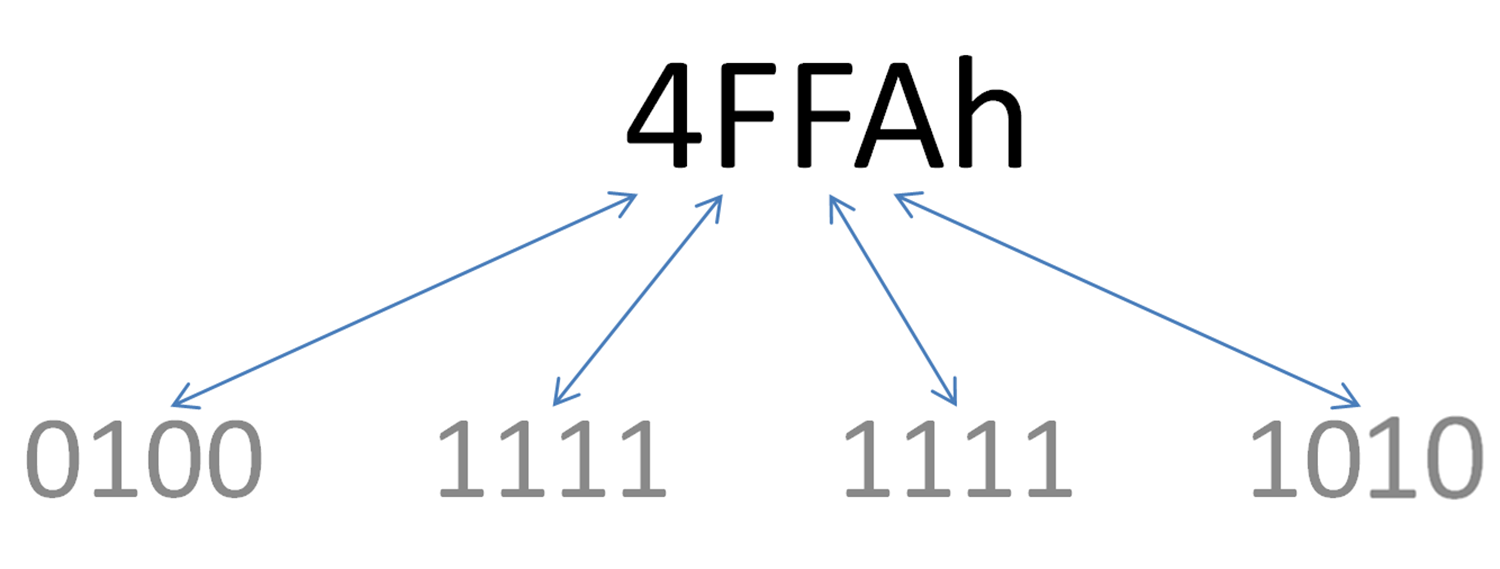
\includegraphics[scale=0.25]{Labo3_4FFA.PNG}
\end{center}

\subsection{Remarque :}
On indique qu’un nombre est hexadécimal en le précédant de 0x, en le terminant par la lettre h (cfr figure plus haut) ou encore en lui ajoutant un indice "16".


\subsection{Conversion hexadécimal => décimal}
Le principe est le même que pour la conversion décimal => binaire (procédure itérative), mais en utilisant les puissances de 16 plutôt que les puissances de 2 et en introduisant une division pour trouver le chiffre correspondant à un poids donné (car ce chiffre peut varier entre 0 et 15 et non uniquement entre 0 et 1).\\

Pour $3287_{10}$, cela donne:
\vspace{2mm}
\begin{itemize}
\item $3287 < 4096 (= 16^3)$ => chiffre hexadécimal $0$ pour $16^3$ – il reste toujours $3287$
\item $3287 > 256 (= 16^2)$ => diviser $3287$ par $256$ pour trouver le chiffre hexadécimal de poids $16^2$ : $3287/256=12,83$ => le chiffre hexadécimal de poids $16^2$ est $12_{10}$ c'est-à-dire $C_{16}$ - il reste: $3287-12.256 = 215$
\item $215 > 16 (= 16^1)$ => diviser $215$ par 16 pour trouver le chiffre hexadécimal de poids $16^1$ : $215/16=13,4375$ => le chiffre hexadécimal de poids $16^1$ est $1310$ c'est-à-dire $D_{16}$ - il reste: $215-13.16 = 7$
\item $7 < 16 (= 16^1)$ => 7 est le chiffre hexadécimal de poids $16^0$
\item => le résultat est $3287_{10} = 0CD7_{16} = 0CD7h = 0x0CD7$
\end{itemize}

\subsection{Conversion binaire => hexadécimal et hexadécimal => binaire}
Ces conversions sont plus faciles car il suffit de remplacer directement chaque chiffre hexadécimal par 4 chiffres binaires (bits) ou inversement (en constituant les bits par groupes de 4 en partant des bits de poids les plus faibles): voir l'exemple avec 4FFAh en haut de cette page.


\subsection{Exercices (PRIOR)}
\Question{0}
{
%question
\textit{Assurez vous que vous savez compter en hexadécimal.}
}
{%assistant
Voir tableau de la page suivante.
}

\Question{0}
{
%question
\textit{Donnez les représentations décimales et binaires des nombres hexadécimaux suivants : 0x0E, 0xA2, 0x0FE1, 0xAAAD.}
}
{%assistant
\begin{itemize}
\item 0x0E : $14_{10}=00001110_{2}$
\item 0xA2 : $162_{10}=10100010_{2}$
\item 0x0FE1 : $4065_{10}=0000111111100001_{2}$
\item 0xAAAD : $43693_{10}=1010101010101101_{2}$
\end{itemize}
}

\Question{0}
{
%question
\textit{Donnez la représentation hexadécimale des nombres binaires suivants : 0101, 1010111, 00101001, 10000110}
}
{%assistant
\begin{itemize}
\item 0101 : 0x05
\item 01010111 : 0x57
\item 00101001 : 0x29
\item 10000110 : 0x86

\end{itemize}
}

\subsection{Tableau récapitulatif des 3 bases}
Les 16 premières lignes du tableau ci-dessous (encadré) sont très utiles pour les conversions de tous types:
\begin{center}
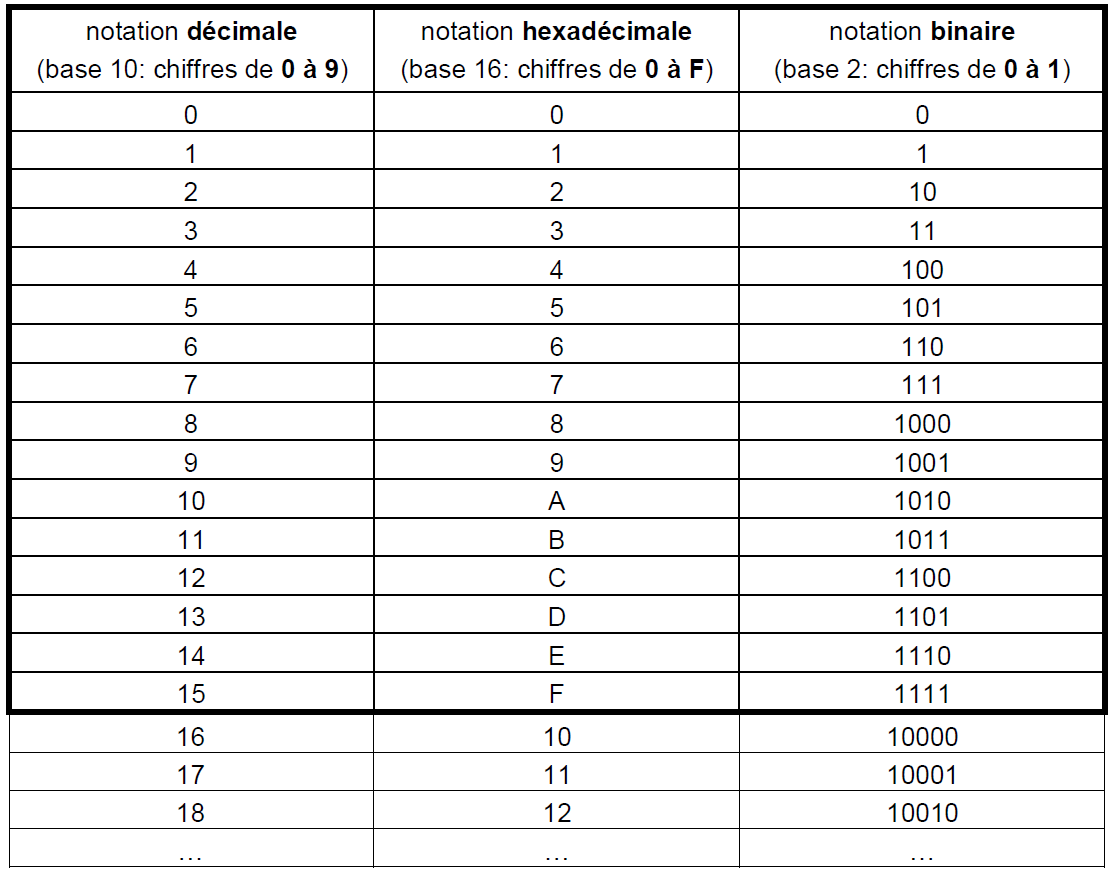
\includegraphics[scale=0.6]{Labo3_Tabrecap.png}
\end{center}

\section{Représentation des caractères sous forme ASCII}
Les caractères, comme toutes les données en informatique, sont représentés sous forme de mots binaires. Néanmoins le codage de l'information est différent\footnote{Par exemple, le mot 4Eh représente le nombre 78 s’il est interprété comme un entier, mais désigne le caractère N lorsque l’on considère la norme ASCII}, et il a notamment fallu se mettre d'accord sur un standard international dans ce domaine.\\

La norme ASCII (American Standard Code for Information Interchange) définit le codage binaire de 127 caractères tels que les chiffres arabes, les lettres latines majuscules et minuscules, quelques symboles de ponctuation et des commandes de contrôle de terminal informatique. Les caractères codés en ASCII sont stockés sur 8 bits (1 octet). Le tableau ci-dessous donne la correspondance de ces caractères en représentation décimale et hexadécimale.\\

Cette norme est à la base de beaucoup d’autres normes comme l’ISO 8859-1 qui ajoute le codage pour 127 autres caractères comme les caractères accentués de la langue française et allemande.
\begin{center}
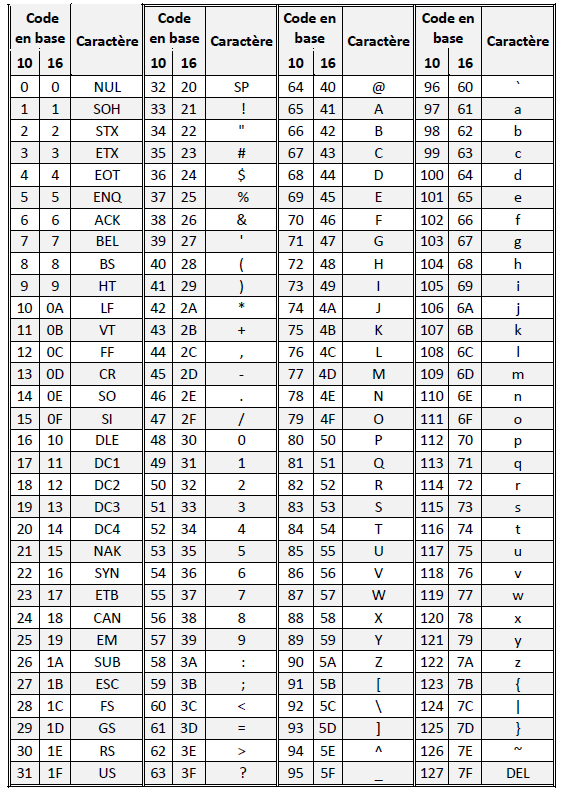
\includegraphics[scale=1]{Labo3_ASCII.png}
\end{center}

\subsection{Exercices}
\Question{0}
{
%question
\textit{Donnez la représentation hexadécimale en codage ASCII de la phrase « Les labos d’electronique sont amusants ! »}
}
{%assistant
4C 65 73 20 6C 61 62 6F 73 20 64 27 65 6C 65 63 74 72 6F 6E 69 71 75 65 20 73 6F 6E 74 20 61 6D 75 73 61 6E 74 73 20 21
}

\Question{0}
{
%question
\textit{Une mémoire contient les mots binaires ci-dessous (notés en hexadécimal). Traduisez ce texte au moyen du code ASCII (les espaces entre les nombres hexadécimaux ne doivent pas être pris en compte dans la traduction):\\
4C 65 73 20 61 73 73 69 73 74 61 6E 74 73 20 73 6F 6E 74 20 67 65 6E 69 61 75 78 2E}
}
{%assistant
Les assistants sont geniaux.
}


\section{Les circuits de mémoire}
Une mémoire est un circuit capable de stocker une certaine quantité d'information sous forme numérique:
\begin{itemize}
\item une mémoire de 1 bit est appelée bistable
\item une mémoire de 1 mot est appelée registre
\end{itemize}

Par ailleurs il existe de nombreux types de mémoires capables de stocker de quelques Kmots à quelques Gmots (voire Tmots): mémoires à semi-conducteur RAM et ROM, mémoires FLASH, etc. Comme ce type de mémoires permet le stockage de plusieurs mots, la notion d'adresse (emplacement d'un mot particulier dans la mémoire) est indispensable. Une telle mémoire possède donc:
\begin{itemize}
\item un bus de données (pour véhiculer l'information)
\item un bus d'adresse (pour véhiculer l'adresse de l'information)
\item un bus de commande (quelques bits pour gérer l'interaction avec les autres circuits)
\end{itemize}
On trouvera à l'annexe B des exemples de circuits de mémoire réels, avec quelques détails de fonctionnement. Cette annexe est donnée à titre d'information.

 \ifthenelse{\boolean{corrige}}{\newpage}{}
\subsection{Exercices (PRIOR)}
\Question{0}
{
%question
\textit{Combien de mots peut contenir une mémoire acceptant 14 bits d’adresse?}
}
{%assistant
$2^{14}$ mots (un mot peut contenir un nombre arbitraire de bits)
}

\Question{0}
{
%question
\textit{Combien de bits d’adresse doit posséder une mémoire dans laquelle on veut pouvoir stocker au moins 68000 octets ? Quel est le nombre maximum d’octets que peut contenir ce circuit (c-à-d sa taille réelle) en octets, Koctets et en bits?}
}
{%assistant
En considérant des mots de 1 octet, il faut minimum $17$ bits. En effet, $2^{16}=65536<68000<131072=2^{17}$.\\
Ce circuit peut donc contenir $2^{17}=131072$ octets, soit $\frac{131072}{1024}=128Ko$, soit $128\times 8= 1024 Kbits$, ou encore $1024\times 1024=1048576\ bits$.
}

\Question{0}
{
%question
\textit{Quelle doit être la taille d’une mémoire dans laquelle on veut stocker 4000 mots de 16 bits si cette mémoire stocke des octets ?}
}
{%assistant
1 mot demande 2 octets => 8192 (8K).
}

\Question{0}
{
%question
\textit{Quelle doit être la taille d’une mémoire dans laquelle on veut stocker 4000 mots de 14 bits si cette mémoire n’accepte que des octets?}
}
{%assistant
Pour la facilité on choisit en général de prendre 2 octets pour un mot (2 bits ne seront donc pas utilisés) => 8K.
}

\Question{0}
{
%question
\textit{Un système mesurant une température à une fréquence de 100Hz doit pouvoir garder en mémoire les mesures effectuées pendant les 5 dernières secondes. Donnez la taille minimale de la mémoire RAM du système si une mesure fait 1 octet ? Quelle sera la taille réelle du circuit RAM de ce système ?}
}
{%assistant
Il faut mémoriser 500 octets => taille de 512 octets
}


\section{Opérations logiques}
Les 7 opérations logiques de base sont rappelées à la figure ci-dessous.\\
Les schémas de brochage des circuits logiques courants sont disponibles en Annexe~\ref{ANNEXE C}.
\begin{center}
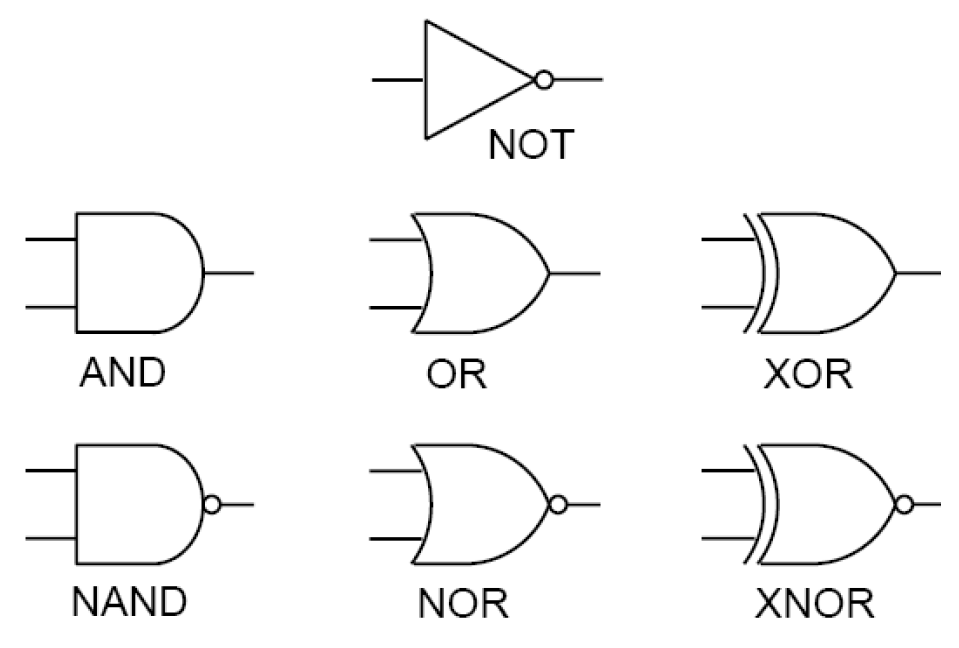
\includegraphics[scale=0.4]{Labo3_Porteslogiques.png}
\end{center}


\subsection{Exercices (PRIOR)}
\Question{0}
{
%question
\textit{Donnez la table de vérité d’une porte logique NAND. Réalisez physiquement ce circuit sur protoboard au moyen d’un circuit 74HC00. Testez son bon fonctionnement à l’aide des boutons du
protoboard et de l’hélice mise à votre disposition.}\\
}
{%assistant
$$X=\overline{A.B}=\overline{A}+\overline{B}$$
\begin{center}
		\begin{tabular}{|c|c|c|}
			\hline
            A&B&X\\
            \hline
            \hline
			0&0&1\\
			0&1&1\\
			1&0&1\\
			1&1&0\\
			\hline
		\end{tabular}
	\end{center}
}

\Question{0}
{
%question
\textit{Schématiser un circuit ayant le même comportement qu’une porte AND à l’aide de deux portes logiques NAND. Réalisez physiquement ce circuit sur protoboard au moyen d’un circuit 74HC00.\\
Testez son bon fonctionnement à l’aide des boutons du protoboard et de l’hélice mise à votre
disposition.}
}
{%assistant
\begin{center}
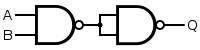
\includegraphics[scale=1]{Labo3_NAND.png}
\end{center}

$$X=\overline{\overline{A.B}}=A.B$$
\begin{center}
		\begin{tabular}{|c|c|c|}
			\hline
            A&B&Q\\
            \hline
            \hline
			0&0&0\\
			0&1&0\\
			1&0&0\\
			1&1&1\\
			\hline
		\end{tabular}
	\end{center}
}


\Question{0}
{
%question
\textit{Donnez la table de vérité du circuit suivant:
\begin{center}
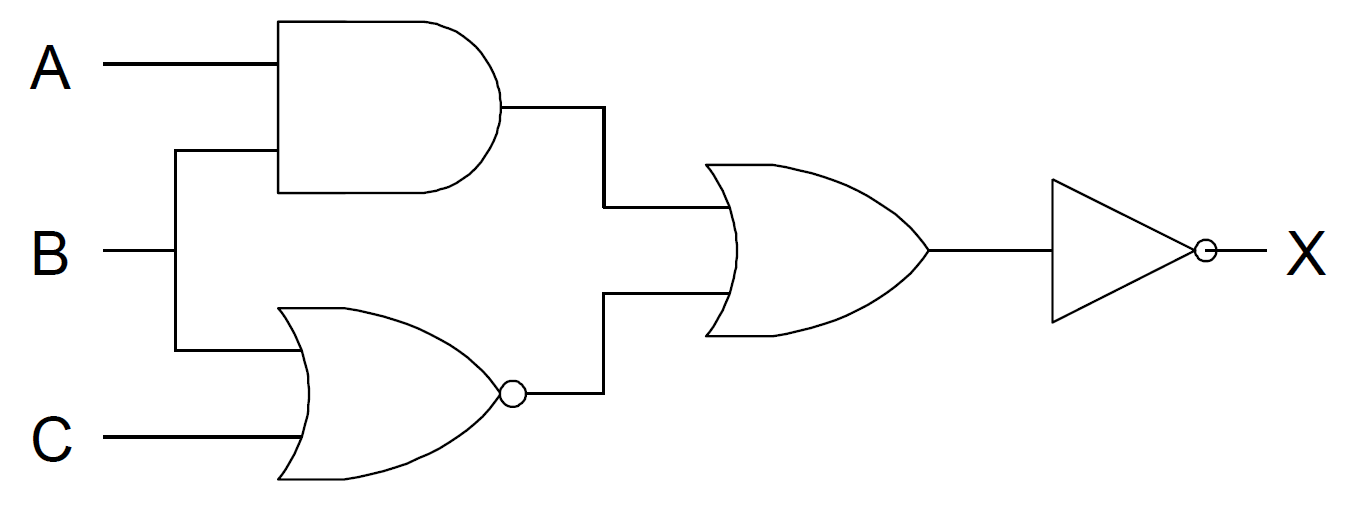
\includegraphics[scale=0.25]{Labo3_Logique_Ex1.png}
\end{center}
}
}
{%assistant

$$X=\overline{A.B+\overline{(B+C)}}$$

%\begin{table} [h]
	\begin{center}
		\begin{tabular}{|c|c|c|c|}
			\hline
            A&B&C&X\\
            \hline
            \hline
			0&0&0&0\\
			1&0&0&0\\
			0&1&0&1\\
			1&1&0&0\\
			0&0&1&1\\
			1&0&1&1\\
			0&1&1&1\\
			1&1&1&0\\

			\hline
		\end{tabular}
	\end{center}
%	\caption{Methods}
%	\label{Methods}
%	\end{table}
}

\Question{0}
{
%question
\textit{Vérifiez, en dressant sa table de vérité, que le circuit ci-dessous est un voteur (expliquez pourquoi ce nom):
\begin{center}
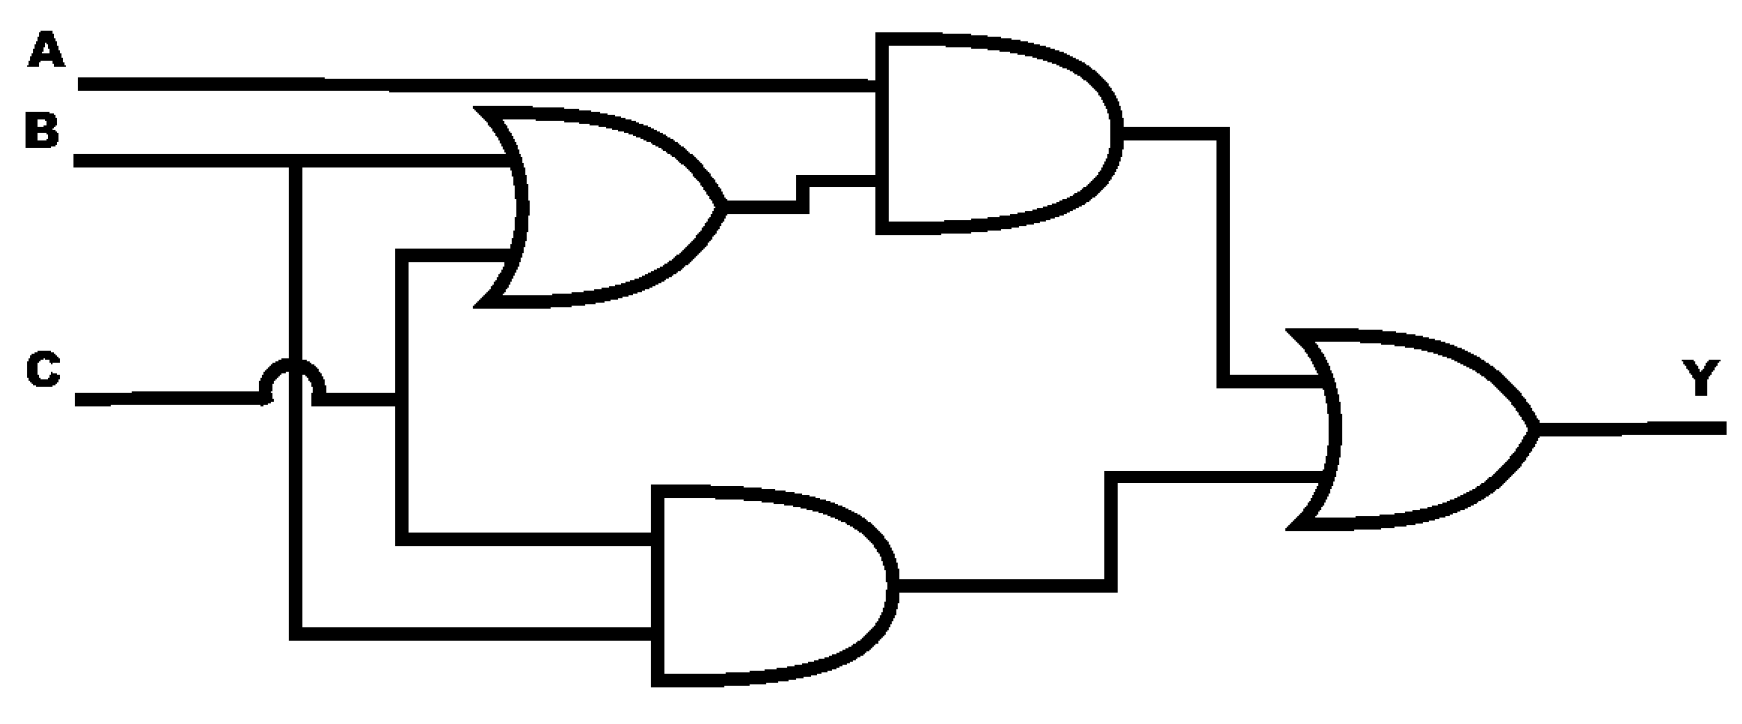
\includegraphics[scale=0.25]{Labo3_Logique_Ex2.png}
\end{center}
Réalisez physiquement ce circuit sur protoboard au moyen de circuits 74HC00 (NAND) et 74HC32 (OR), et testez son bon fonctionnement.}
}
{%assistant
\begin{center}
Y=(A.(B+C))+(B.C)
\end{center}
%\begin{table} [h]
	\begin{center}
		\begin{tabular}{|c|c|c|c|}
			\hline
            A&B&C&X\\
            \hline
            \hline
			0&0&0&0\\
			1&0&0&0\\
			0&1&0&0\\
			1&1&0&1\\
			0&0&1&0\\
			1&0&1&1\\
			0&1&1&1\\
			1&1&1&1\\

			\hline
		\end{tabular}
	\end{center}
%	\caption{Methods}
%	\label{Methods}
%	\end{table}
}
%
\Question{0}
{
%question
\textit{Complétez le chronogramme du circuit suivant, en considérant que la porte « NOT » a un temps de
propagation de 10ns et que la porte « AND » a un temps de propagation de 20ns.
\begin{center}
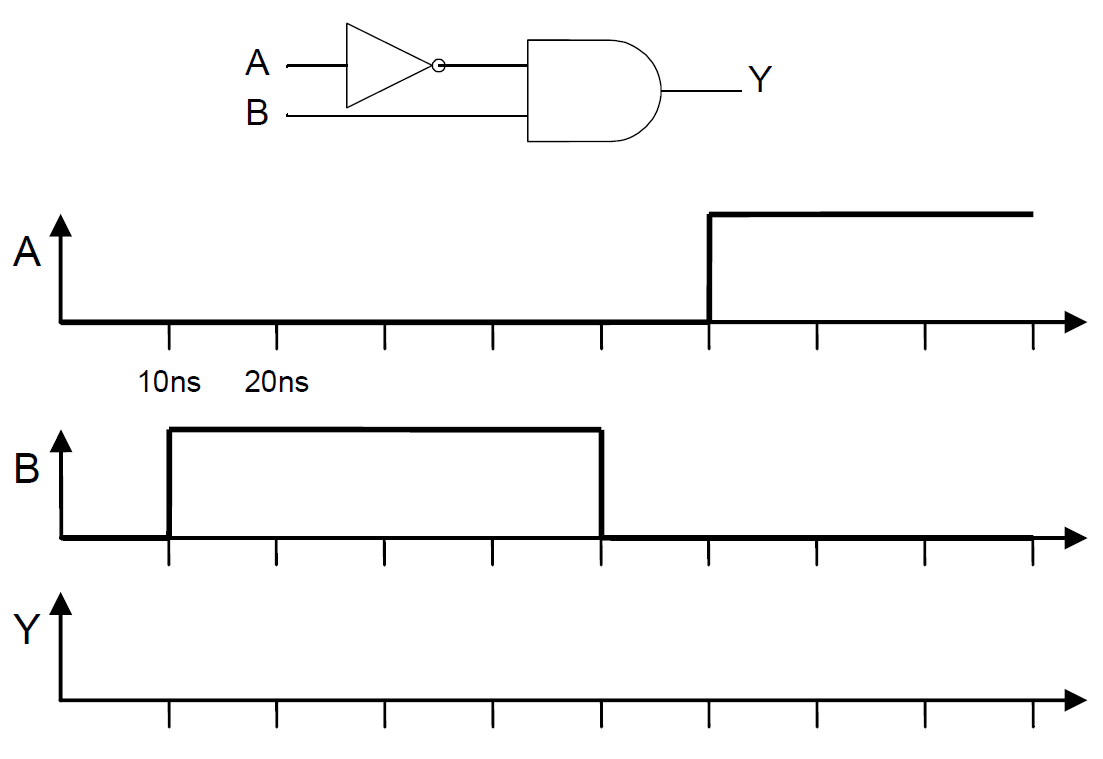
\includegraphics[scale=0.65]{Labo3_Chronogramme.png}
\end{center}
}
}
{%assistant
\begin{center}
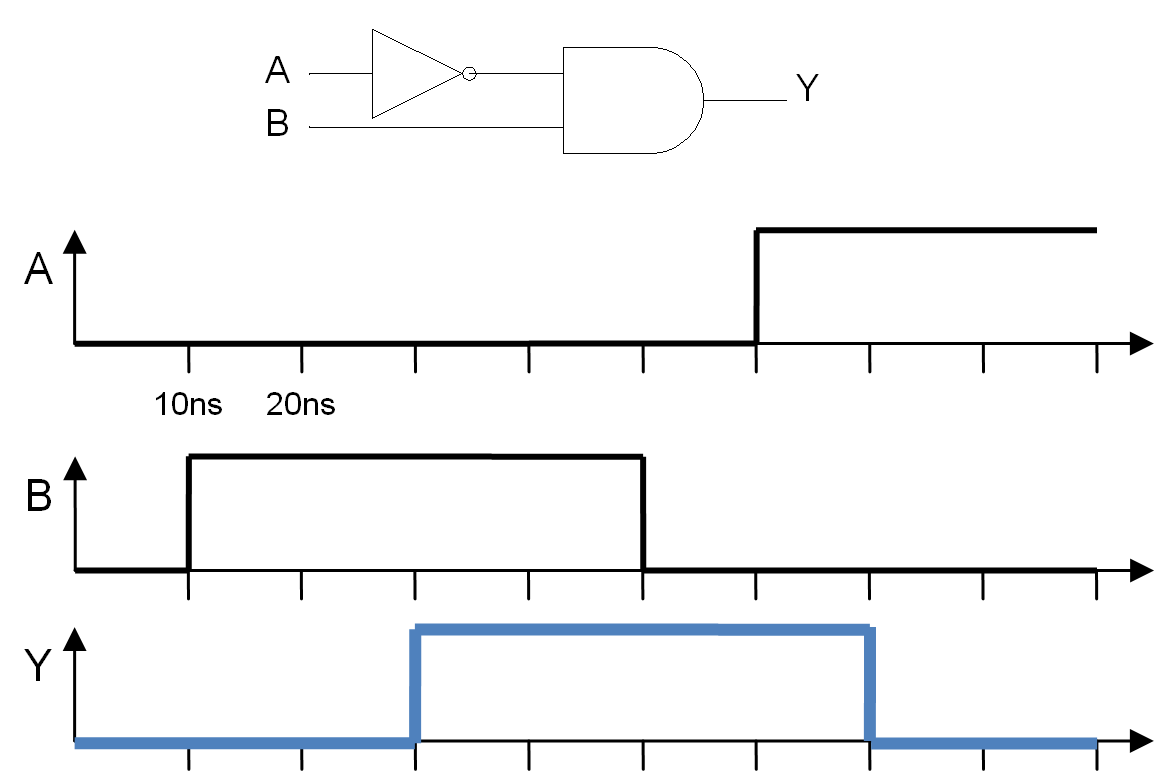
\includegraphics[scale=0.6]{Labo3_Chronogramme_sol.png}
\end{center}
}

\section{Mémorisation: réalisation d'un bistable}\footnote{Le but est ici de vous faire réaliser un bistable pour vous faire comprendre les principes de base du numérique, en particulier le stockage d'une information logique au moyen de circuits et de tensions qui sont en fait analogiques. En situation réelle, vous utiliserez des mémoires "toutes faites".}
Les bistables sont des circuits très employés en électronique numérique en raison de leurs multiples
applications. Leur première fonction est de mémoriser une information logique.
Les bistables sont des circuits séquentiels, c'est-à-dire que, contrairement aux circuits combinatoires, leur état de sortie ne dépend pas uniquement des entrées mais également de leur état de sortie précédant.

\subsection{Un bistable élémentaire}
Ci-dessous est représenté sous 2 formes différentes le bistable le plus simple.
\begin{center}
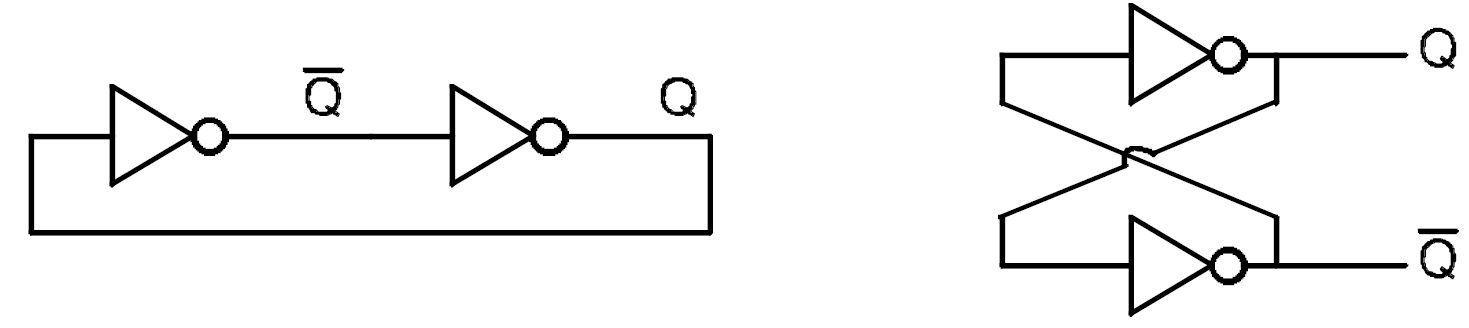
\includegraphics[scale=0.35]{Labo3_Bistableelementaire.png}
\end{center}


Ce bistable possède 2 états stables (d'où son nom):
\begin{itemize}
\item soit $Q$ est à l'état haut (H) et $\overline{Q}$ est à l'état bas (L)
\item soit $Q$ est à l'état bas (L) et $\overline{Q}$ est à l'état haut (H)
\end{itemize}

Ce circuit est donc une mémoire. Malheureusement, il est difficile de modifier son état autrement
qu'en court-circuitant une des sortie à un état déterminé: il n'y a en effet pas d'entrée à ce circuit.

\subsection{Amélioration}
Imaginons que l'on dispose d'inverseurs dont on peut mettre la sortie dans un état déterminé. Par
exemple l'inverseur suivant :
\begin{center}
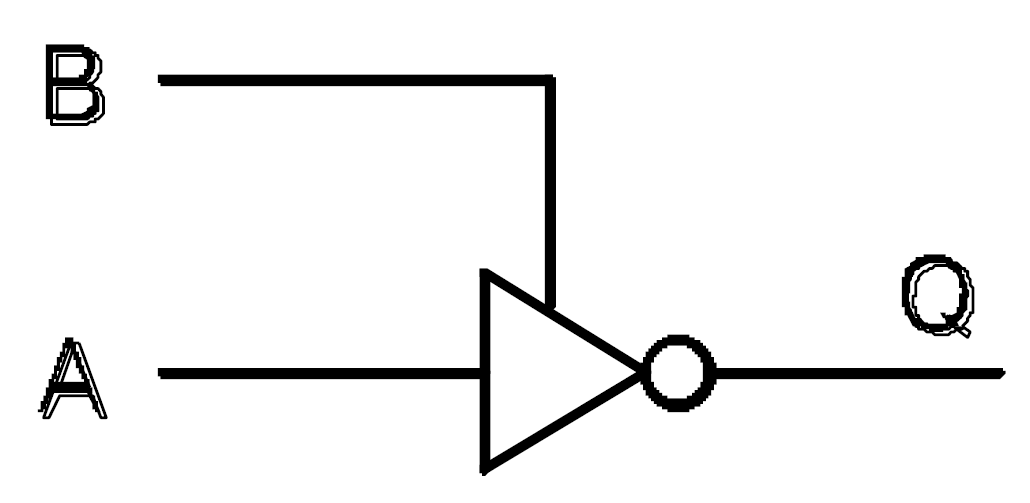
\includegraphics[scale=0.15]{Labo3_Amelioration1.png}
\end{center}

\begin{itemize}
\item si B est à l'état bas, alors Q est l'inverse de A (inversion normale de A)
\item si B est à l'état haut, alors Q est à l'état bas (par exemple)
\end{itemize}

On peut alors réaliser le montage suivant :
\begin{center}
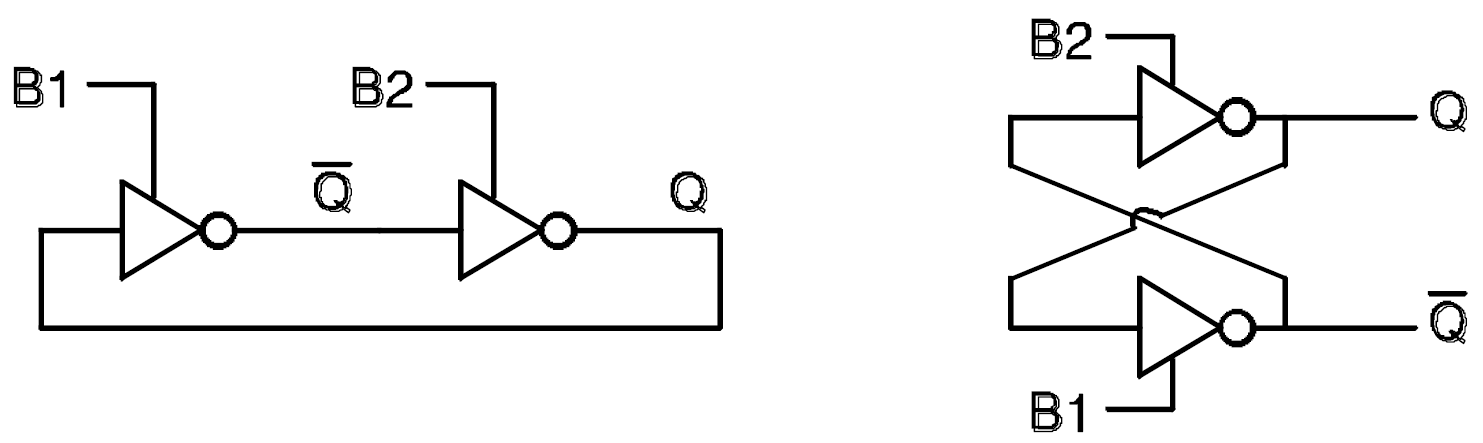
\includegraphics[scale=0.35]{Labo3_Amelioration2.png}
\end{center}

On peut maintenant réaliser les opérations suivantes :
\vspace{3mm}
\begin{itemize}
\item mettre l'entrée B2 à l'état haut et l'entrée B1 à l'état bas : la sortie $Q$ est alors mise à l'état bas.
\item mettre l'entrée B2 à l'état bas et l'entrée B1 à l'état haut : la sortie $Q$ est alors mise à l'état haut.
\item mettre les 2 entrées B1 et B2 à l'état bas : le circuit reste dans sont état précédant : c'est la
mémorisation.
\end{itemize}
\vspace{3mm}
Le cas où les 2 entrées B1 et B2 sont à l'état haut n'est pas intéressant : il force les 2 sorties $Q$ et $\overline{Q}$ à
l'état bas. C'est un cas qui n'est pas cohérent: c'est pourquoi on l'appellera indésirable.

\subsection{Bistable R-S}
En fait, on connaît, sans le savoir, des éléments logiques qui répondent à l'inverseur spécial vu ci-dessus.\\
Prenons par exemple la porte NOR (Non OU).
\begin{center}
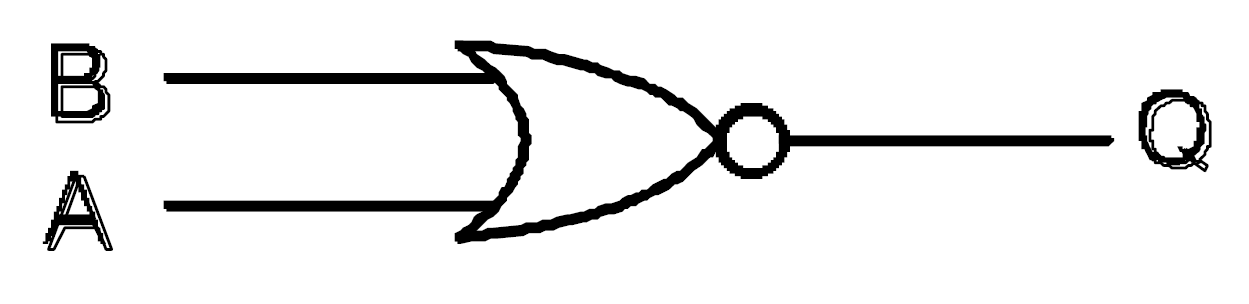
\includegraphics[scale=0.2]{Labo3_NOR.png}
\end{center}

Cette porte répond parfaitement à la table de vérité de l'inverseur spécial : si son entrée B est à l'état haut, la sortie Q est forcée à l'état bas ; sinon, la sortie Q est l'inverse de l'entrée A.\\


Construisons alors le bistable à partir de ces portes et renommons (R, S) les entrées (B1, B2).
\begin{center}
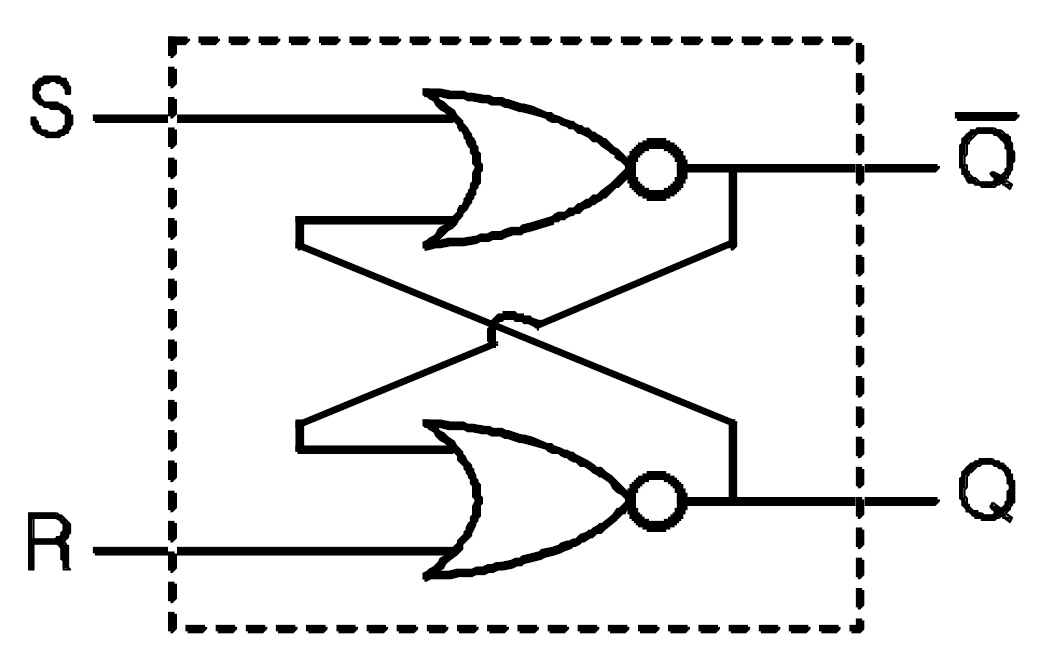
\includegraphics[scale=0.3]{Labo3_RS_NOR.png}
\end{center}

\begin{itemize}
\item Pour mettre la sortie Q à l'état bas, il suffit d'appliquer un état haut à l'entrée R (Reset : mise à l'état bas)
et un état bas à l'entrée S (Set : mise à l'état haut)
\item Pour mettre la sortie Q à l'état haut, il suffit d'appliquer un état haut à l'entrée S (Set : mise à l'état haut)
et un état bas à l'entrée R (Reset : mise à l'état bas)
\item Pour être en mémorisation, il suffit d'appliquer un état bas aux 2 entrées.
\end{itemize}
\vspace{3mm}
Si on appelle l'état bas le niveau inactif et l'état haut le niveau actif, alors on peut dire :
\vspace{3mm}
\begin{itemize}
\item pour mettre le bistable dans un état déterminé, il suffit d'appliquer un niveau actif à l'entrée
correspondante.
\item pour mettre le bistable en mémorisation, il suffit de ne mettre aucun niveau actif
\item l'état indésirable à lieu lorsqu'on demande au bistable en même temps une mise à l'état haut et une mise à l'état bas.
\end{itemize}

\subsection{Table de vérité du bistable R-S}
Si on n'est pas convaincu par les développements précédents, on peut écrire la table de vérité du
bistable R-S :
\begin{center}
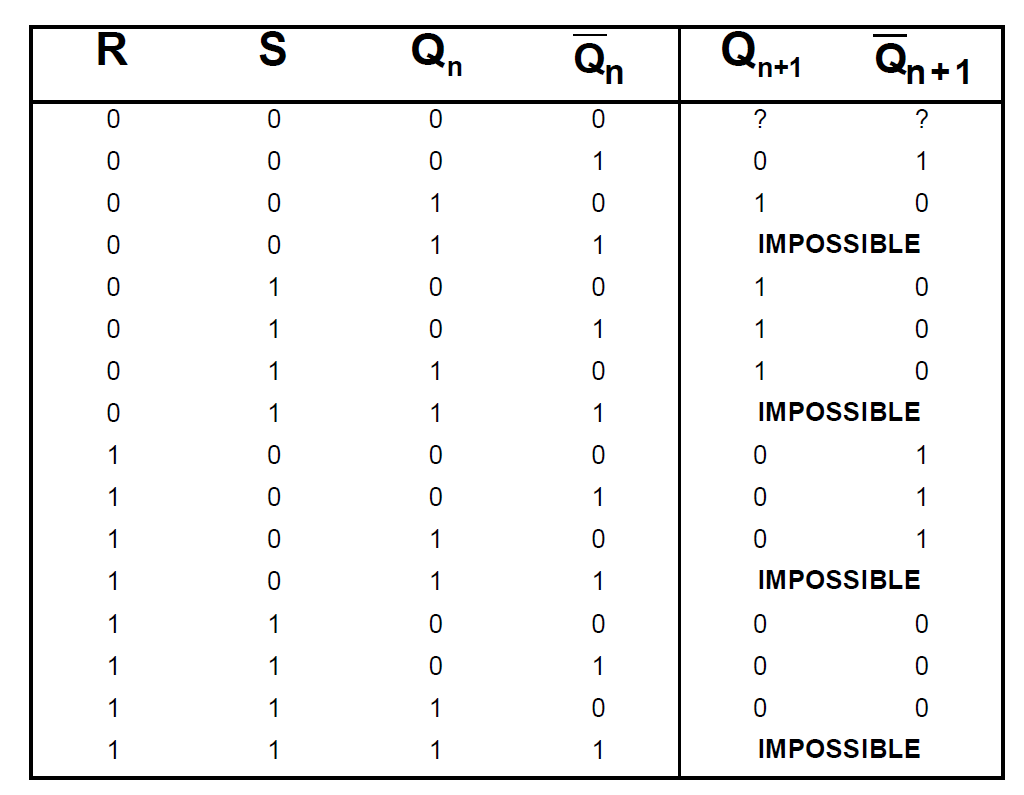
\includegraphics[scale=0.6]{Labo3_RS_tab1.png}
\end{center}

En entrée de la table, on met les 2 sorties stables à l'instant t et les entrée que l'on applique à ce
même instant. En sortie de la table, on détermine l'état des 2 sorties à l'instant t+tp, c-à-d après le
temps de propagation du bistable.\\

Cette table de vérité peut être simplifiée, en effet, les états impossibles ne sont pas à prendre en
considération puisqu'ils ne seront jamais rencontrés. Il ne faut cependant pas confondre état
impossible en entrée (lignes impossibles) et état indéterminé en sortie (ligne 1). La table devient:
\begin{center}
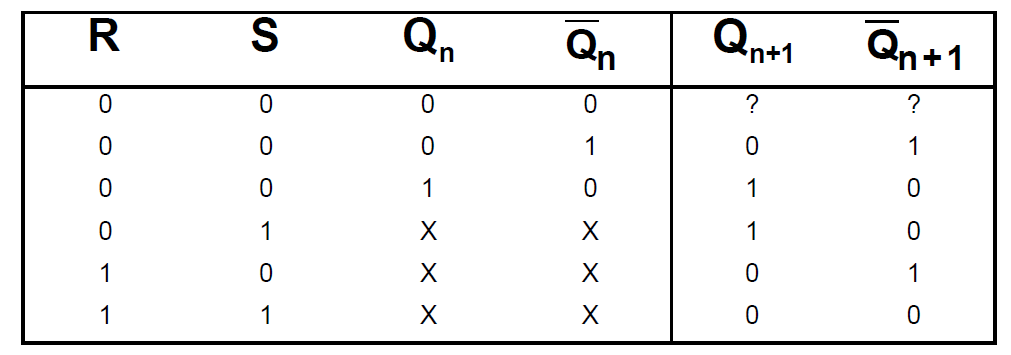
\includegraphics[scale=0.6]{Labo3_RS_tab2.png}
\end{center}

Le dernier état est évidement indésirable puisqu'il rend égales des sorties normalement
complémentaires (l'ordre donné au bistable est incohérent). Si on évite cet état, on peut supprimer la
dernière ligne du tableau ainsi que la première. On peut alors simplifier cette table pour avoir :
\begin{center}
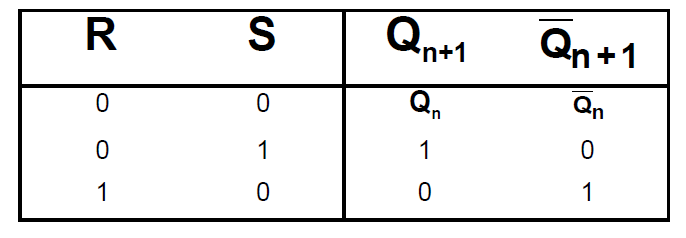
\includegraphics[scale=0.6]{Labo3_RS_tab3.png}
\end{center}

De cette table, on retire heureusement les mêmes conclusions que précédemment.\\


La méthode par table de vérité est assez lourde dans son entièreté. Il vaut donc mieux essayer
d'établir directement la table simplifiée comme vu précédemment.

\subsection{Exercice: Réalisation d'un bistable R-S (PRIOR)}
Réaliser le schéma suivant à l'aide de portes logiques.
\begin{center}
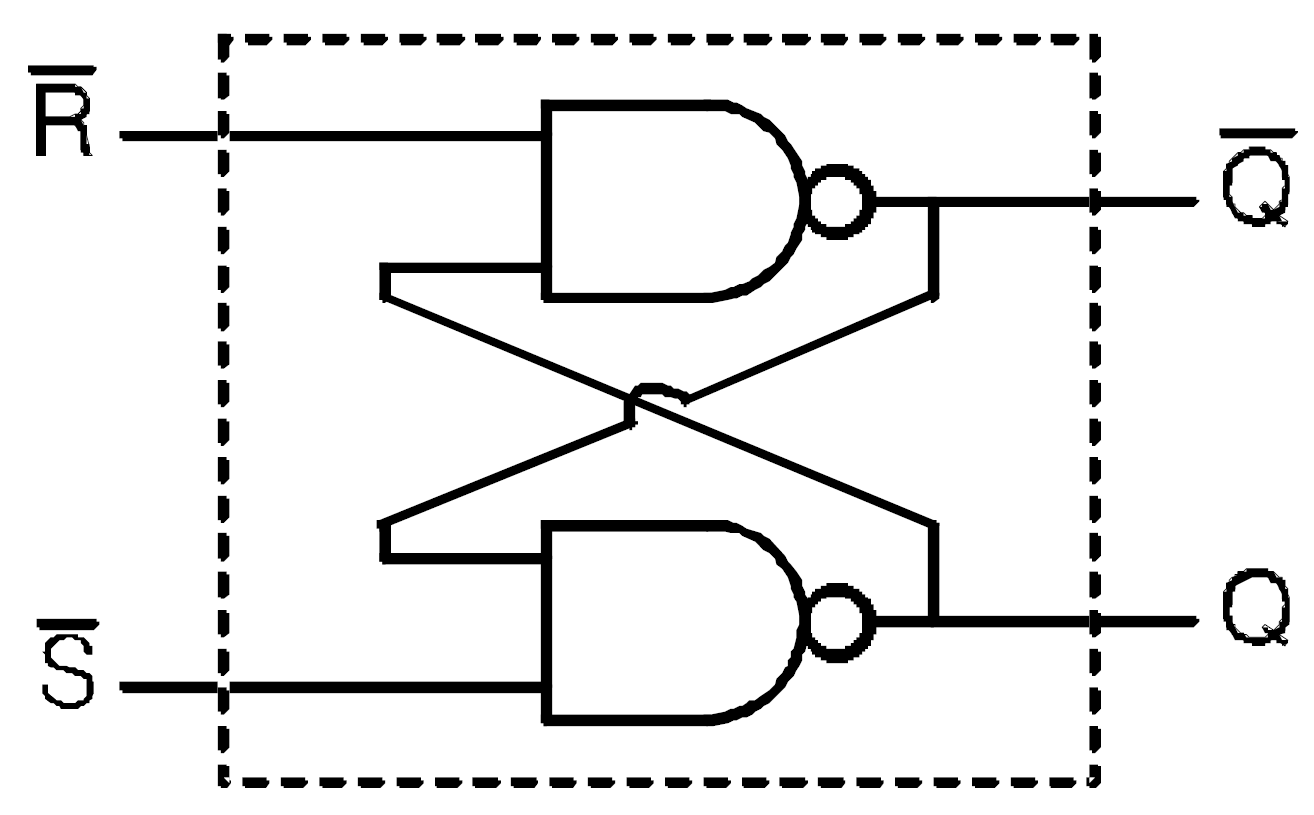
\includegraphics[scale=0.2]{Labo3_RS.png}
\end{center}

\Question{0}
{
%question
\textit{Quel est l'état des entrées qui assure la fonction de mémorisation?}
}
{%assistant
1 sur l’entrée Set et 1 sur l’entrée Reset.
}

\Question{0}
{
%question
\textit{Que faut-il appliquer au circuit pour réaliser un Set ou Reset ?}
}
{%assistant
Fonction Set : S=0 (actif à l’état bas) et R=1 (inversement pour le Reset).
}

\Question{0}
{
%question
\textit{Quelle est l'anomalie des sorties lorsque les deux entrées sont à l'état bas ?}
}
{%assistant
Les deux sorties sont actives (état interdit).
}

\Question{0}
{
%question
\textit{Donner à chaque valeur des entrées (R, S) une appellation parmi les suivantes :
[mémorisation], [mise à 0], [mise à 1], [indésirable]}
}
{%assistant
ATTENTION! Les entrées sont actives à l’état bas, c’est-à-dire qu’un 0 les rend actives et qu’un 1 les rend inactives.
	\begin{center}
		\begin{tabular}{|c|c|c|c|c|}
			\hline
            R&S&$Q_{n}$&$-Q_{n}$&\\
            \hline
            \hline
			0&0&(1)&(1)&[indésirable]\\
			0&1&0&1&[mise à 0]\\
			1&0&1&0&[mise à 1]\\
			1&1&$Q_{n-1}$&$-Q_{n-1}$&[mémorisation]\\
			\hline
		\end{tabular}
	\end{center}
}

\Question{0}
{
%question
\textit{Justifier appellation R-S. (R : Reset S : Set); Quel est le niveau logique actif de ces 2 entrées?
Pourquoi parle-t-on d'entrées en logique inverse ?}
}
{%assistant
Activer l’entrée Set impose un 1 ; activer l’entrée Reset impose à 0.\\
Car les entrées sont actives à l’état bas.
}

\Question{0}
{
%question
\textit{Que pourrait-il se passer si on passe de l'état [mise à 1] à l'état [mémorisation] en passant
transitoirement par l'état [indésirable] ?}
}
{%assistant
On pourrait rester dans l’état indésirable.\\
Dans un cas réel, on se retrouvera soit à l’état [mise à 0] ou [mise à 1] car les deux entrées peuvent difficilement changer simultanément pour mémoriser l’état [indésirable].
}

\subsection{Exercice : Bistable R-S avec Enable (entrée d'activation) (PRIOR)}
Modifier le montage précédent comme suit :
\begin{center}
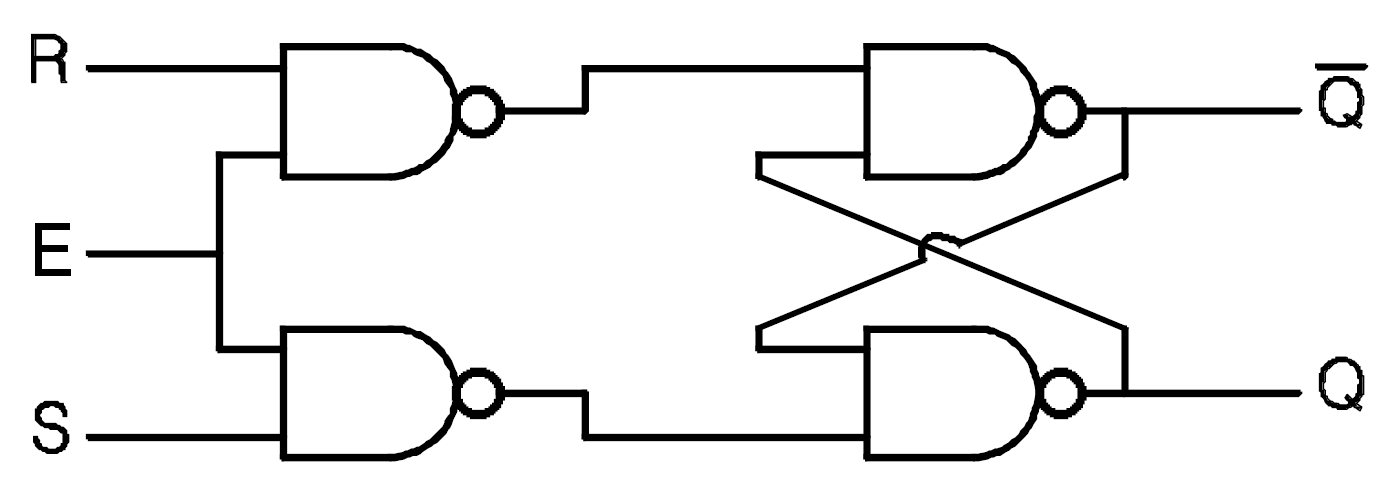
\includegraphics[scale=0.3]{Labo3_RSavecE.png}
\end{center}

\Question{0}
{
%question
\textit{Réalisez physiquement ce circuit sur protoboard au moyen d’un circuit 74HC00 (NAND). Testez
son bon fonctionnement à l’aide des boutons du protoboard et de l’hélice mise à votre disposition.}
}
{%assistant
}

\Question{0}
{
%question
\textit{Mettre en évidence l'avantage de l'entrée E (Enable) du point de vue des modifications des
entrées R et S.}
}
{%assistant
Le Set ou le Reset ne sont possibles que lorsque Enable est à 1.
}

\subsection{Exercice: D Latch}
Le D Latch répond au schéma suivant :

\begin{center}
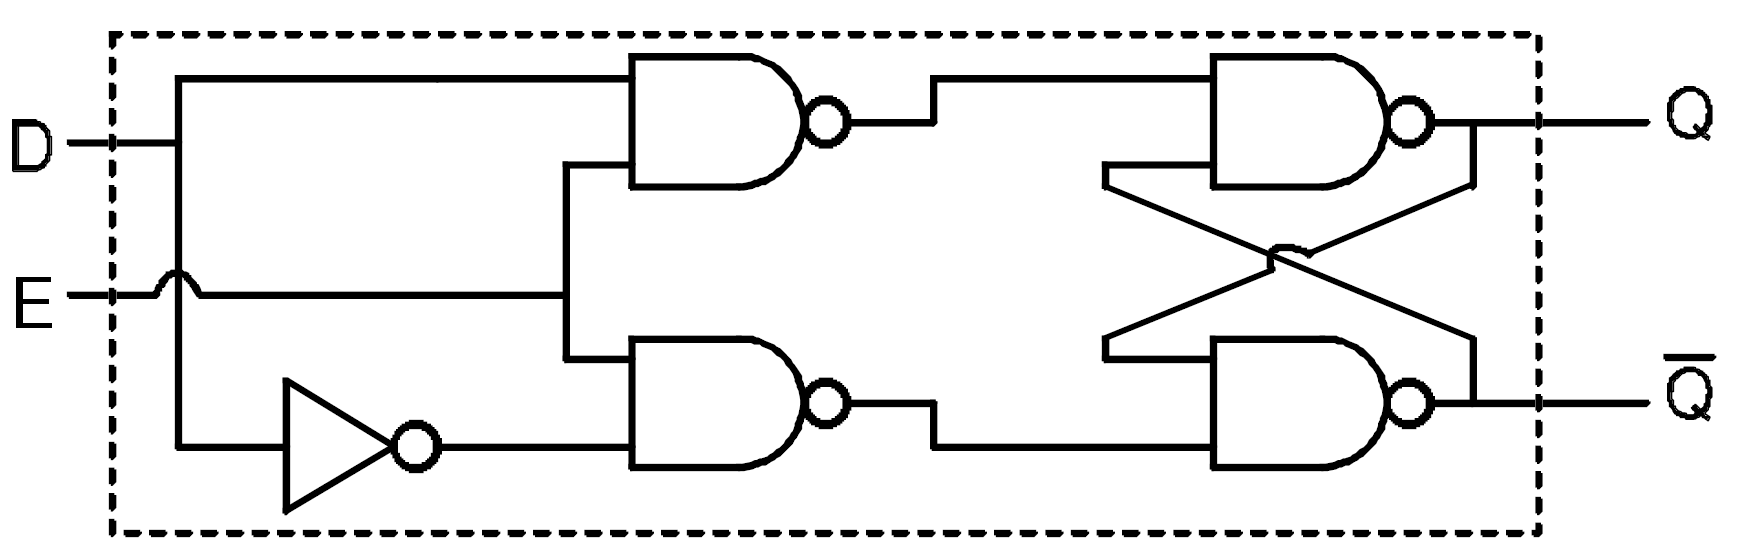
\includegraphics[scale=0.2]{Labo3_DLatch.png}
\end{center}

L'inverseur en tête du montage a pour effet de supprimer l'état illicite du bistable R-S de sortie.
\Question{0}
{
%question
\textit{Réaliser le D LATCH à l'aide de portes logiques.}
}
{%assistant
}
\Question{0}
{
%question
\textit{Déterminer son fonctionnement. (table de vérité simplifiée)}
}
{%assistant
	\begin{center}
		\begin{tabular}{|c|c|c|c|c|}
			\hline
            D&E&$Q_{n}$&$-Q_{n}$&\\
            \hline
            \hline
			0&0&$Q_{n-1}$&$-Q_{n-1}$&[mémorisation]\\
			1&0&$Q_{n-1}$&$-Q_{n-1}$&[mémorisation]\\
			0&1&0&1&[mise à 0]\\
			1&1&1&0&[mise à 1]\\
			\hline
		\end{tabular}
	\end{center}
}
\Question{0}
{
%question
\textit{Vérifier que votre circuit reproduit bien le fonctionnement attendu}
}
{%assistant
}
\Question{0}
{
%question
\textit{Peut-on, à votre avis, modifier D n'importe quand ?}
}
{%assistant
Seulement quand l’entrée E (Enable) est active
}


\newpage
\section*{ANNEXE A: Codage binaire des nombres entiers négatifs (pour info)}
\label{ANNEXE A}
\subsection*{Les nombres binaires en complément à 2}
En binaire la manière de représenter les nombres entiers négatifs est le codage en "complément à 2". Sur 8 bits (un octet) :
\begin{itemize}
\item les entiers positifs de 0 à 127 se représentent classiquement par les nombres binaires allant de 00000000 à 01111111 ;
\item les entiers négatifs allant de -1 à –128 se représentent par les codes binaires allant respectivement de 11111111 à 10000000.
\end{itemize}
Le bit de poids le plus élevé donne donc le signe du nombre : 1= négatif, 0=positif.
Attention cependant: pour un nombre négatif, les 7 bits de poids faible utilisent un autre codage que le codage en positi (voir ci-dessous).

\subsection*{Conversion décimal => binaire complément à 2}
Pour les nombres positifs la manière de coder est la même que pour les nombres binaires.
Pour les nombres négatifs : par exemple, pour trouver le code en complément à 2 correspondant à –67 vous devez :\\
\begin{itemize}
\item trouver le nombre binaire à 8 bits correspondant à 67 : 01000011 ;
\item prendre son complément à 1 (inverser tous les bits): 10111100 ;
\item ajouter 1.
\end{itemize}
Donc, –67 se représente par 10111101.

\subsection*{Conversion binaire complément à 2 => décimal}
Si le bit de poids le plus élevé est à 1, le nombre est négatif et vous devez effectuer les opérations inverses :
\begin{itemize}
\item trouver le complément à 2 pour trouver la valeur absolue ;
\item trouver l’entier positif correspondant au nombre binaire obtenu ;
\item ne pas oublier de mettre un "-" devant.
\end{itemize}



\section*{ANNEXE B: Exemples de circuits de mémoire (pour info)}
\vspace{-0.1cm}
\label{ANNEXE B}

\subsection*{La RAM}
La figure 1a montre un circuit intégré de mémoire RAM statique de 8Ko, le HM6264 de Hitachi (le chiffre 64 signifie que c’est une mémoire de 64Kbits, donc 8Ko).\\

\begin{center}
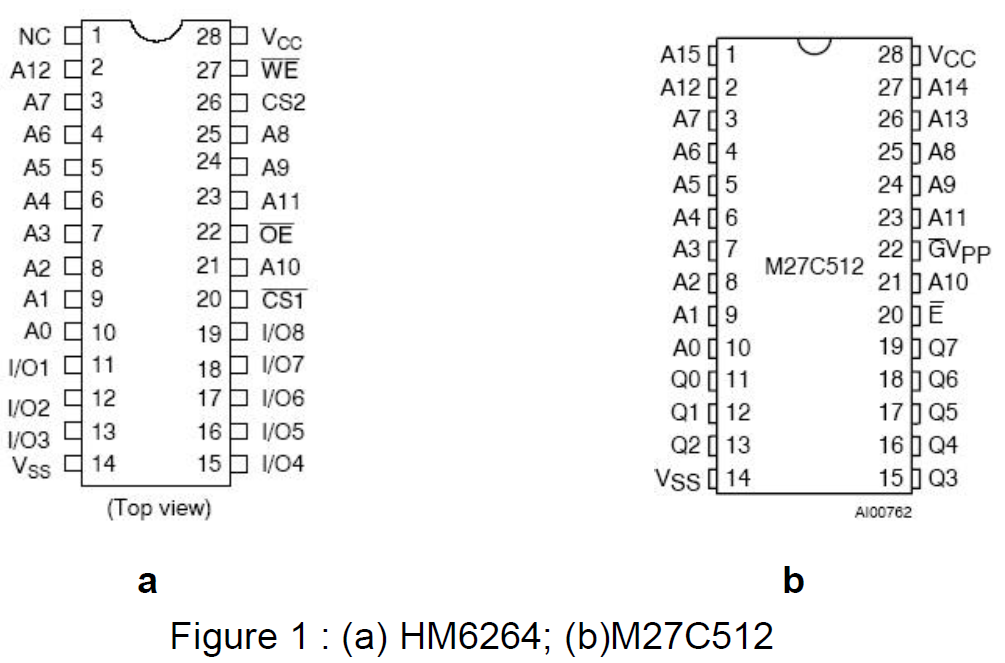
\includegraphics[scale=0.6]{Labo3_AnnexeB.png}
\end{center}

En plus des pattes d’alimentation (VCC et VSS), cette mémoire possède des pattes d'entrées/sorties\footnote{Un point d'exclamation devant le nom d'un signal (ex: !A) signifie que ce signal est actif à l'état bas (équivalent à la notation "surlignée" A, difficile à utiliser dans un traitement de texte). "Activer" un tel signal consiste donc bien à lui donner la valeur 0 (sa valeur par défaut, correspondant à une absence d'activité, valant 1).}.\\

Celles-ci peuvent être divisées en trois types selon leur fonction :

\begin{itemize}
\item \textbf{les entrées d’adresse} (A12 …A0) : entrées indiquant l’emplacement mémoire (octet) auquel on s’adresse ;
\item \textbf{les entrées/sorties des données} (I/O8 .. I/O1) : dans le cas d’une lecture, ce sont des sorties donnant l’octet contenu dans la mémoire à l’emplacement indiqué par le bus d’adresse et dans le cas d’une écriture, ce sont des entrées par lesquelles on fournit l’octet à enregistrer à l’emplacement indiqué par le bus d’adresse.
\item \textbf{les entrées de contrôle} :
	\begin{itemize}
	\item !WE (Write Enable): indique que l’on veut effectuer une opération d’écriture à l’emplacement indiqué par les entrées d’adresses ;
	\item !CS1 et CS2 (Chip Select 1 et 2): signaux permettant d’activer le circuit, si un des signaux est désactivé les pins I/O8 .. I/O1 sont désactivés quels que soient les états des autres pattes d’E/S ;
	\item !OE (Output Enable): indique que l’on veut effectuer une opération de lecture à l’emplacement indiqué par les entrées d’adresses.
	\end{itemize}
\end{itemize}

\subsection*{Opérations de lecture et d’écriture en RAM}
Pour \textbf{lire} dans la RAM, il faut :
\begin{itemize}
\item activer les signaux CS ;
\item placer l’adresse sur les entrées A12 .. A0 ;
\item activer le signal !OE.
\end{itemize}
Après un petit temps de réponse appelé temps d’accès de la mémoire, l’octet situé dans la mémoire à l’adresse indiquée par les bits d’adresse A12 .. A0 est disponible sur les sorties I/O8 .. I/O1.
Pour \textbf{écrire} dans la RAM, il faut:
\begin{itemize}
\item activer le ou les signaux CS ;
\item placer l’adresse sur les entrées A12 .. A0 ;
\item placer l’octet à enregistrer sur les entrées I/O8 .. I/O1 ;
\item activer le signal !WE (les autres signaux restant inactifs).
\end{itemize}
Afin que le mot soit correctement enregistré, il est nécessaire de maintenir cet état pendant un certain temps (nécessaire à la stabilisation des tensions dans la mémoire).

\subsection*{La ROM}
La figure 1b montre un circuit UVPROM de 64K. Les différences par rapport à la RAM sont les suivantes :\\
\begin{itemize}
\item les pins Q7 .. Q0 sont les équivalents des pins I/O8 .. I/O1 de la RAM, mais ici elles ne fonctionnent qu’en sortie !
\item !E : signal enable permettant d’activer ou de désactiver le circuit.
\end{itemize}

Pour lire dans l’UVPROM, il faut :
\begin{itemize}
\item activer le signal !E ;
\item placer l’adresse sur les entrées A12 .. A0.
\end{itemize}
Après un petit temps de réponse appelé temps d’accès de la mémoire, l’octet se trouvant à l’adresse indiqué par les bits d’adresse A12 .. A0 se retrouve sur les sorties Q7 .. Q0.

\section*{Annexe C : Brochage de circuits logiques courants}
\vspace{-0.1cm}
\label{ANNEXE C}
\begin{center}
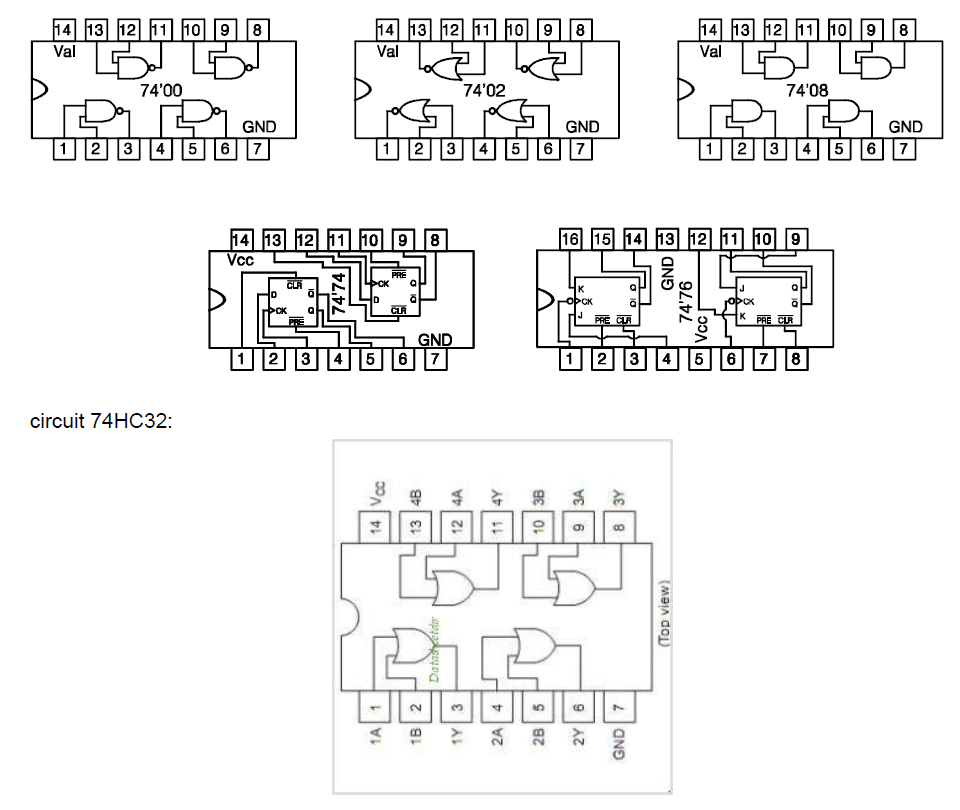
\includegraphics[scale=0.8]{Labo3_AnnexeC.png}
\end{center}

\endinput
